\chapter{Elektromagnetiese bestraling}\fancyfoot[LO,RE]{Fisika: Golwe, Klank en Lig}
    \setcounter{figure}{1}
    \setcounter{subfigure}{1}
    \label{459e2bef85baf867f5850bc8338cad3a}
         \section{Wat is \textsl{elektromagnetiese bestraling}?}
    \nopagebreak
  Die eerste voorbeeld van elektromagnetiese (EM) bestraling is lig. Almal is vertroud met lig in die alledaagse lewe, en mens kan voorwerpe slegs sien wanneer lig daarvan af weerkaats en jou oog binnedring. Hierdie eienskap alleen van lig maak dit betekenisvol genoeg om van lig te leer. Daar is egter ook baie ander toepassings van EM bestraling. Dit word elektromagneties genoem, want daar is elektriese en magnetiese velde wat saam die bestraling opmaak. Ons sal hierdie konsep bietjie later in meer diepte ondersoek. 

\chapterstartvideo{VPefg}

  Alhoewel lig in die alledaagse lewe nie baie ooglopende spesiale eienskappe blyk te h\^e nie, moet mens tog let op die volgende: 
\begin{itemize}
 \item \textbf{ 'n wye spektrum}: Die lig wat ons kan sien (sigbare EM bestraling) is slegs  'n klein deel van die bestaande EM bestralings spektrum. 
 \item \textbf{die natuur se spoedgrens}: Niks beweeg vinniger as die spoed van lig nie.  
 \item \textbf{golf geaardheid}: Alle EM bestraling het die vermoee om op te tree soos  'n golf. 
 \item \textbf{partikel geaardheid}: Alle EM bestraling het die vermoee om op te tree soos  'n partikel.
 \item \textbf{Geen medium benodig}: EM bestraling kan bestaan sonder die teenwoordigheid van  'n medium waardeur dit hoef te beweeg, selfs al het dit  'n golf geaardheid.
\end{itemize}

Twee belangrike konsepte om van kennis te dra, soos hierbo genoem:
\begin{enumerate}[noitemsep, label=\textbf{\arabic*}. ]
 \item golf geaardheid sonder  'n nodige medium om in te beweeg, en 
 \item being beide  'n partikel en  'n golf. 
\end{enumerate}
Ons sal die bogenoemde in die volgende afdelings bespreek, en in selfs meer detail in Graad 11 en 12 ingaan. 

    \label{m38777*cid3}
            \section{Golf aard van EM bestraling}
            \nopagebreak
      \label{m38777*id186686}As jy kyk na  'n klomp miere wat loop van een punt na  'n ander, dan lyk dit na  'n dun ononderbroke swart lyn. Maar as jy egter die lyn miere van nader bekyk, sal jy sien dat die lyn miere bestaan uit duisende aparte miere.\par 
      \label{m38777*id187029}Lig en alle ander tipes elektromagnetiese bestraling blyk ook  'n ononderbroke golf aanvanklik te wees, maar wanneer mens eksperimente met lig uitvoer, begin mens agterkom dat lig beide golf sowel as partikel eienskappe het. Net soos die individuele miere, kan die lig ook opgemaak wees uit individuele bondels energie, of kwantum lig.\par 
      \label{m38777*id187035}Lig het beide golf-agtige en partikel-agtige eienskappe (golf-partikel dualiteit), maar slegs die een of die ander word getoon, afhangende van die aard van die eksperiment wat verrig word.  'n Golf-tipe eksperiment toon die golf natuur, en  'n partikel-tipe eksperiment toon die partikel natuur.  'n Mens kan nie die golf en die partikel geaardheid op dieselfde tydstip toets nie.  'n Lig partikel staan bekend as  'n foton.\par 




\Definition{Foton}{ 'n Foton is  'n kwantum (energie pakkie) lig.} 



\subsection*{Velde}
            \nopagebreak
      \label{m38777*id187125}\textit{Versnellende belading} skei elektromagnetiese golwe af.  'n Veranderende elektriese veld genereer  'n magnetiese veld and  'n veranderende magnetiese veld genereer  'n elektriese veld. Hierdie is die beginsel agter die voorplanting van elektromagnetiese golwe, aangesien elektromagnetiese golwe, anders as klankgolwe, nie  'n medium benodig waardeur dit hoef te beweeg nie.  

\mindsetvid{Animation of electric fields}{VPeka}

EM golwe plant voort wanneer  'n elektriese veld, ossillerend op een vlak,  'n magnetiese veld produseer wat op een vlak ossilleer teen  'n 90 grade hoek daarmee, wat dan weer  'n ossillerende magnetiese veld produseer, en so voorts.   Die voorplanting van die elektromagnetiese golwe kan beskyf word as \textsl{wedersydse induksie}.\par Ons gebruik $E$ om elektriese velde aan te dui, en $B$ om magnetiese velde aan te dui\par

Hierdie wedersydse wederbarende velde beweeg deur  'n vakuum teen  'n konstante spoed van $3\ensuremath{\times}{10}^{8}\phantom{\rule{0.166667em}{0ex}}\text{m}\ensuremath{\cdot}{\text{s}}^{-1}$, voorgestel deur $c$.\par 
      \label{m38777*eip-43}Alhoewel  'n elektromagnetiese golf deur  'n vakuum kan beweeg, kan dit ook deur  'n medium soos water en lug beweeg. Wanneer  'n elektromagnetiese golf egter deur  'n medium beweeg, sal dit stadiger beweeg as wanneer dit deur  'n vakuum sou beweeg.\par \label{m38777*id187191}
    \setcounter{subfigure}{0}
	\begin{figure}[H] % horizontal\label{m38777*id187194}
    \begin{center}

\begin{pspicture}(-4,-4)(3,4)
\psset{Alpha=30}
\pstThreeDCoor[nameY=$B$,nameZ=$E$,linecolor=black,xMin=-4,yMin=-4,zMin=-4]
\parametricplotThreeD[xPlotpoints=200,linecolor=blue,linewidth=1.5pt,plotstyle=curve,linestyle=dashed](-180,180){%
    t 60 div
    3 2.5 t mul cos mul
    0}
\parametricplotThreeD[xPlotpoints=200,linecolor=red,linewidth=1.5pt,plotstyle=curve](-180,180){%
    t 60 div
    0
     -3 2.5 t mul cos mul
    }
\end{pspicture}
\caption{
  'n Diagram wat die wedersydse wederbarende elektriese veld (soliede rooi lyn) and magnetiese veld (blou stippeltyn) aandui.
}

 \end{center}
 \end{figure}       
      \par \label{m38777*eip-808}Aangesien EM bestraling  'n golf is, sal die volgende formula steeds van toepassing wees: \par \label{m38777*eip-181}\nopagebreak\noindent{}
    \begin{equation}
    v=f\ensuremath{\cdot}\lambda
      \end{equation}
      \label{m38777*eip-601}Behalwe dat ons ons $v$ kan vervang met $c$:\par \label{m38777*eip-194}\nopagebreak\noindent{}
    \begin{Formula}
    c=f\ensuremath{\cdot}\lambda
      \end{Formula}
      \par
            \label{m38777*eip-923}\vspace{.5cm} 
      \noindent
      \begin{wex}{EM bestraling I}{
      \label{m38777*id187899}Bereken die frekwensie van  'n elektromagnetiese golf met  'n golflengte van $4,2\ensuremath{\times}{10}^{-7}$ m.}
      { 
      \westep{Golf Formule}
      \label{m38777*id187948}Ons gebruik die formula: $c=f\lambda $ om frekwensie te bepaal. Die spoed van lig is konstant $3\ensuremath{\times}{10}^{8}$m/s.\par 
      \westep{Bereken}  
    \begin{equation}
    \begin{array}{ccc}\hfill c& =& f\lambda \hfill \\ \hfill 3\ensuremath{\times}{10}^{8}& =& f\ensuremath{\times}4,2\ensuremath{\times}{10}^{-7}\hfill \\ \hfill f& =& 7,14\ensuremath{\times}{10}^{14}\text{Hz}\hfill \end{array}
      \end{equation}}    \end{wex}
 
      \begin{wex}{EM Bestraling II}{
      \label{m38777*id188123}  'n Elektromagnetiese golf het  'n golflengte van $200\phantom{\rule{3.33333pt}{0ex}}\text{nm}$. Wat is die frekwensie van die radiasie?}{
      \westep{Wat weet ons?}
      \label{m38777*id188341} Onthou dat alle bestraling beweeg teen die spoed van lig ($c$) in  'n vakuum.
Aangesien die vraag nie spesifiek aandui deur watter materie die golf beweeg nie, is dit veilig vir ons om te aanvaar dat die golf beweeg deur  'n vakuum. 
Ons kan twee eienskapp van die bestraling identifiseer - $wavelength\phantom{\rule{3.33333pt}{0ex}}\left(200\phantom{\rule{3.33333pt}{0ex}}\text{nm}\right)$ and speed ($c$).\par 
    \westep{Pas die golf formule toe} 
    \begin{equation}
    \begin{array}{ccc}\hfill c& =& f\lambda \hfill \\ \hfill 3\ensuremath{\times}{10}^{8}& =& f\ensuremath{\times}200\ensuremath{\times}{10}^{-9}\hfill \\ \hfill f& =& 1.5\ensuremath{\times}{10}^{15}\phantom{\rule{4pt}{0ex}}\text{Hz}\hfill \end{array}
      \end{equation}}    \end{wex}

\section{Elektromagnetiese spektrum}
            \nopagebreak
EM bestraling word geklassifiseer in tipes, afhangend van die frekwensie van die golf: hierdie tipes sluit in, in volgende van toenemendheid van die frekwensie, radio golwe, mikrogolwe, infra-rooi bestraling, sigbare lig, ultra-violet bestraling, x-strale and gamma strale. \par 
            \nopagebreak
      
            \mindsetvid{Electromagnetic spectrum}{VPemp}


      \label{m38778*id187332}Table \ref{Table:EMSpectrumRanges} Lys die golflengte en frekwensie reeks van die afdeldings van die elektromagnetiese sprektrum.\par 
    % \textbf{m38778*uid8}\par
          \begin{table}[H]
    % \begin{table}[H]
    % \\ '' '0'
        \begin{center}
      \label{m38778*uid8}
    \noindent
    
      \begin{tabular}[t]{|l|l|l|}\hline
                \textbf{Kategorie}
               &
                \textbf{Golflengte Reeks(nm)}
               &
                \textbf{Frekwensie Reeks (Hz)}
              % make-rowspan-placeholders
     \tabularnewline\cline{1-1}\cline{2-2}\cline{3-3}
      %--------------------------------------------------------------------
        gamma strale &
        $\lessthan{}$1 &
                $\greatthan{}3\ensuremath{\times}{10}^{19}$
              % make-rowspan-placeholders
     \tabularnewline\cline{1-1}\cline{2-2}\cline{3-3}
      %--------------------------------------------------------------------
        X-strale &
        1-10 &
        $3\ensuremath{\times}{10}^{17}$-$3\ensuremath{\times}{10}^{19}$% make-rowspan-placeholders
     \tabularnewline\cline{1-1}\cline{2-2}\cline{3-3}
      %--------------------------------------------------------------------
        ultra-violet lig &
        10-400 &
        $7,5\ensuremath{\times}{10}^{14}$-$3\ensuremath{\times}{10}^{17}$% make-rowspan-placeholders
     \tabularnewline\cline{1-1}\cline{2-2}\cline{3-3}
      %--------------------------------------------------------------------
        sigbare lig &
        400-700 &
        $4,3\ensuremath{\times}{10}^{14}$-$7,5\ensuremath{\times}{10}^{14}$% make-rowspan-placeholders
     \tabularnewline\cline{1-1}\cline{2-2}\cline{3-3}
      %--------------------------------------------------------------------
        infra-rooi &
        700-${10}^{5}$ &
        $3\ensuremath{\times}{10}^{12}$-$4,3\ensuremath{\times}{10}^{19}$% make-rowspan-placeholders
     \tabularnewline\cline{1-1}\cline{2-2}\cline{3-3}
      %--------------------------------------------------------------------
        mikrogolf &
                ${10}^{5}-{10}^{8}$
               &
        $3\ensuremath{\times}{10}^{9}$-$3\ensuremath{\times}{10}^{12}$% make-rowspan-placeholders
     \tabularnewline\cline{1-1}\cline{2-2}\cline{3-3}
      %--------------------------------------------------------------------
        radio golwe &
                $\greatthan{}{10}^{8}$
               &
                $\lessthan{}3\ensuremath{\times}{10}^{9}$
              % make-rowspan-placeholders
     \tabularnewline\cline{1-1}\cline{2-2}\cline{3-3}
      %--------------------------------------------------------------------
    \end{tabular}
      \end{center}
    \label{table:EMSpectrumRanges}
    \caption{Elektromagnetiese spektrum}
\end{table}
    \par
      \label{m38778*id188548} Voorbeelde van sommige gebruike van elektromagnetiese golwe word gewys in Tabel \ref{Table:EMUses}.\par 
    % \textbf{m38778*uid9}\par
          \begin{table}[H]
    % \begin{table}[H]
    % \\ '' '0'
        \begin{center}
      \label{m38778*uid9}
    \noindent
    
      \begin{xtabular}[t]{|l|l|}\hline
                \textbf{Kategorie}
               &
                \textbf{Gebruike}
              % make-rowspan-placeholders
     \tabularnewline\cline{1-1}\cline{2-2}
      %--------------------------------------------------------------------
        gamma strale &
        gebruik om die bakterie in malvalekkers dood te maak, sowel as vir die sterilisasie van mediese toerusting		% make-rowspan-placeholders
     \tabularnewline\cline{1-1}\cline{2-2}
      %--------------------------------------------------------------------
        X-strale &
        gebruik om been strukture grafies voor te stel		% make-rowspan-placeholders
     \tabularnewline\cline{1-1}\cline{2-2}
      %--------------------------------------------------------------------
        ultra-violet lig &
        bye kan ultra-violet lig sien, en blomme kom meer helder voor op hierdie frekwensie. % make-rowspan-placeholders
     \tabularnewline\cline{1-1}\cline{2-2}
      %--------------------------------------------------------------------
        sigbare lig &
        word gebruik deur mense om die wereld te bekyk en bestudeer % make-rowspan-placeholders
     \tabularnewline\cline{1-1}\cline{2-2}
      %--------------------------------------------------------------------
        infra-rooi &
        nag visie, hitte sensors, laser metaal snywerk % make-rowspan-placeholders
     \tabularnewline\cline{1-1}\cline{2-2}
      %--------------------------------------------------------------------
        mikro-golf &
        mikrogolf oonde, radar % make-rowspan-placeholders
     \tabularnewline\cline{1-1}\cline{2-2}
      %--------------------------------------------------------------------
        radio golwe &
        radio, televisie uitsendings % make-rowspan-placeholders
     \tabularnewline\cline{1-1}\cline{2-2}
      %--------------------------------------------------------------------
    \end{xtabular}
      \end{center}\label{Table:EMUses}
        \caption{
	  Gebruike van EM Golwe
	}
\end{table}
               \subsubsection*{EM bestraling}
            \nopagebreak
      \label{m38778*id188768}\begin{enumerate}[noitemsep, label=\textbf{\arabic*}. ] 
            \label{m38778*uid10}\item Rangskik die volgende tipes EM bestraling in volgorde van toenemende frekwensie: infra-rooi, x-strale, ultra-violet, sigbare lig en gamma-strale.\newline
\label{m38778*uid11}\item Bereken die frekwensie van  'n EM golf met  'n golflengte van 400~nm.\newline
\label{m38778*uid12}\item Gee  'n voorbeeld van die gebruike van elke tipe EM bestraling, bv. gamma-strale, X-strale, ultra-violet lig strale, sigbare lig, infra-rooi, mikro-golwe en radio en televisie golwe.\newline
\end{enumerate}
    \label{m38778*cid6}
\practiceinfo
 \par \begin{tabular}[h]{cccccc}
 (1.) l23  &  (2.) l2O  &  (3.) l2i  & \end{tabular}

	\begin{figure}[H] % horizontal\label{m38778*uid3}
    \begin{center}
    \rule[.1in]{\figurerulewidth}{.005in} \\
        \label{m38778*uid3!!!underscore!!!media}\label{m38778*uid3!!!underscore!!!printimage}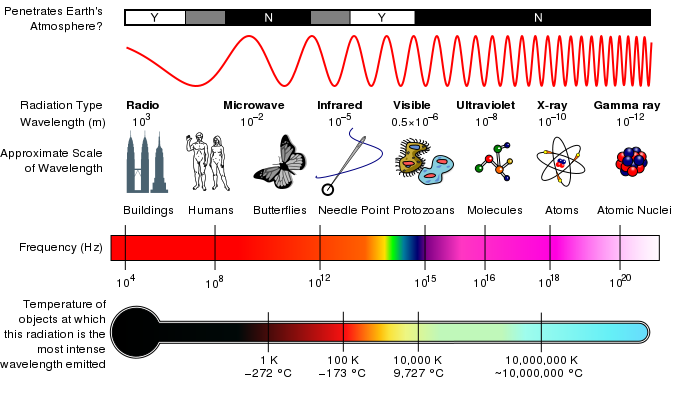
\includegraphics[width=\columnwidth]{col11305.imgs/m38778_EM_Spectrum_Properties_edit.png} % m38778;EM\_Spectrum\_Properties\_edit.png;;;6.0;8.5;
      \label{fig:emspectrum}
      \caption{Die elektromagnetiese spektrum as a funksie van frekwensie. Die verskillende tipes afhangend van golflengte word gewys sowel as alledaagse vergelykings.
	}
    \vspace{.1in}
    \rule[.1in]{\figurerulewidth}{.005in} \\
    \end{center}
 \end{figure}       
      \label{m38778*id187230}EM bestraling laat ons toe om te kan sien. Die frekwensies bestraling wat die menslike oog sensitief voor is, is slegs  'n baie klein deel van al die moontlike frekwensies van EM bestraling. Die volle stel van EM bestraling word genoem die elektromagnetiese sprektrum. Om die konsep te vereenvoudig, word die sprektrum verdeel in onderafdelings, naamlik radio, mikro-golf, infra-rooi, sigbare lig, ultra-violet lig, x-strale en gamma-strale. \par 
      \label{m38778*eip-855}Die EM spektrum is aaneenhoudend (gapingloos) en oneindig. Weens tegnologiese beperkings, kan ons slegs elektromagnetiese bestraling gebruik met golflengtes tussen ${10}^{-14}\text{m}$ en ${10}^{15}\text{m}$.
\label{m38778*secfhsst!!!underscore!!!id117}
           \section{Peneterende vermo\"e van elektromagnetiese bestraling}
            \nopagebreak
      \label{m38779*id189450}Verskillende frekwensies van EM bestraling het verskillende penetrasie vermoens. Byvoorbeeld, as ons die menslike liggaam as objek gebruik, dan word sigbare lig gereflekteer van die oppervlak van die menslike liggaam af, ultra-violet lig (van die son) beskadig die vel, maar x-strale kan die vel en been penetreer en maak foto's van binne die menslike liggaam moontlik. \par 
      \label{m38779*id189457} As ons die energie van sigbare lig vergelyk met die energie van x-strale, dan vind ons dat x-strale het  'n veel hoer frekwensie. Gewoonlik het elektromagnetiese bestraling met  'n hoer frekwensie  'n hoer penetrasie vermo\"e as die met laer frekwensies. \par 
      \label{m38779*id189462} Sommige tipes elektromagnetiese bestraling soos ultra-violet strale, x-strale en gamma-strale is baie gevaarlik. Bestraling afkomstig van hierdie tipes staan bekend as ioniserende bestraling. Ioniserende bestraling dra energie oor soos dit deur materie beweeg, breek molekulere verbindings af en skep ione. \par 
      \label{m38779*id189468} Oormatige blootstelling aan bestraling, insluitende sonlig, x-strale and alle kernkrag bestraling, kan die ontbinding van biologiese weefsel veroorsaak. Gelukkig beskerm die aarde se atmosfeer ons en ander lewende wesens van meeste van die skadelike EM bestraling..\par 
      \label{m38779*uid17}
            \subsubsection*{Ultra-violet (UV) bestraling en die vel}
            \nopagebreak
        \label{m38779*id189482} UVA en UVB is verskillende reekse van frekwensies van (UV) lig. UVA en UVB kan kollageen vesels beskadig wat dan die resultaat het van verhoogde vel veroudering. Oor die algemeen is UVA die minder skadelike een van die twee, alhowel dit bydra tot die veroudering van vel, DNA skade en moontlike vel kanker. Dit penetreer op  'n diep vlak, en veroorsaak nie sonbrand nie. \par 
        \label{m38779*id189490}UVB lig kan vel kanker veroorsaak. Die bestraling affekteer die DNA molekules in die vel se selle, wat dan kan veroorsaak in moontlike kankeragtige mutasies. Die osoonlaag in die atmosfeer beskerm ons teen UVB bestraling. Die verhouding tussen UVB bestraling en kanker is een van die redes vir kommer rakende die afname van osoon in die atmosfeer. \par 
        
\label{m38779*id189495}Die menslike liggaam raak bruin wanneer dit bootgestel word aan  'n matige (afhangend van vel tipe) vlak van bestraling, deur die vrystel van die bruin pigment melanin. Dit help om om UV penetrasie te blok, en voorkom skade aan die meer sensitiewe vel weefsel. Sonbrand-olie blok UV bestraling gedeeltelik en is geredelik beskikbaar. Hierdie produkte het  'n sonbeskermingsfaktor (SBF) aanduiding (gewoonlik aangedui op die houer) wat aandui tot watter mate die produk beskerming bied teen UVB bestraling. Die SBF dui nie aan wat die beskerming is teen UVA bestraling nie. Sommige sonbrand-olie bevat deesdae titanium dioksied wat kan help beskerm teen UVA bestraling. Ander UVA afwerende stowwe gevind in sonbrand-olie sluit in sink dioksied and avobenzone. \par 
\label{m38779*secfhsst!!!underscore!!!id701}
\begin{minipage}{.5\textwidth}
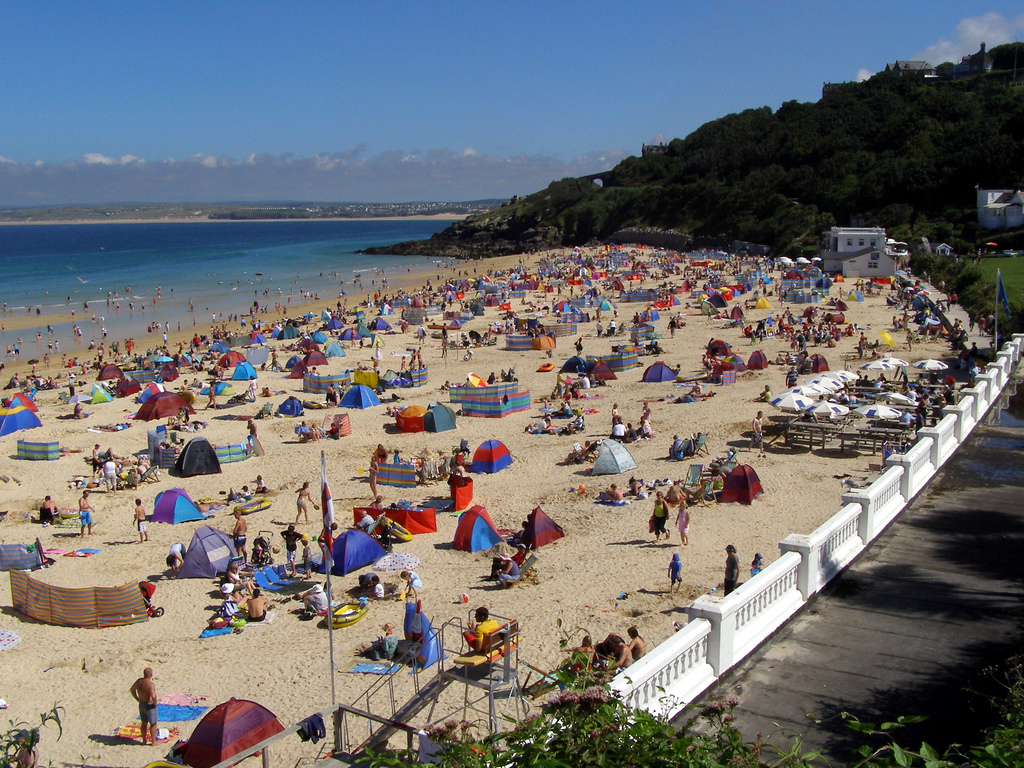
\includegraphics[width=.8\columnwidth]{photos/beach2_treehouse1977.jpg}
\end{minipage}
\begin{minipage}{.5\textwidth}
            \subsubsection*{Wanneer is sonbrand-olie effektief? }
            \nopagebreak
        \label{m38779*id189518}\begin{itemize}[noitemsep]
            \label{m38779*uid18}\item UVB beskerming: Padimate O, Homosalate, Octisalate (octyl salicylate), Octinoxate (octyl methoxycinnamate)
\label{m38779*uid19}\item UVA beskerming: Avobenzone
\label{m38779*uid20}\item UVA/UVB beskerming: Octocrylene, titanium dioksied, sink oksied, Mexoryl (ecamsule)
\end{itemize}
        \label{m38779*id189561}  'n Verdere manier om UV te blok, is deur die dra van spesifieke klere wat beskerm teen die son. Dit is klere wat  'n UPF gradering het wat die beskerming teen beide UVA en UVB beskryf. \par 
      \label{m38779*uid21}
\end{minipage}
            \subsubsection*{Ultra-violet bestraling en die o\"e}
            \nopagebreak
        \label{m38779*id189581}Hoe intensiteit UVB lig kan skade veroorsaak aan die o\"e, en blootstelling kan foto keratitis ("arc eye") veroorsaak, en kan lei tot katarakte en ander mediese toestande. \par 
        \label{m38779*id189586}Beskermende oogtoestelle is voordelig vir diegene wat werk met of blootgestel is ultra-violet bestraling. Gegewe dat die lig die oog kan bereik ook van die kante, is volle oogbeskerm aanbeveelbaar. 
        \label{m38779*id189594} Gewone, onbehandelde brille bied ook tot  'n mate beskerming. Plastiek lense bied meer beskerming as glas lense. Sommige plastike lense materiale soos polie-karbonaat, blok die meeste UV strale. Meeste kontakte lense beskerm die retina deur die absorbsie van UV bestraling. \par 
      \label{m38779*uid22}
      \begin{minipage}{.5\textwidth}
            \subsubsection*{X-strale}
            \nopagebreak
        \label{m38779*id189613}Alhoewel x-strale gebruik word in die mediese veld, kan verlengde blootstelling aan x-strale lei tot sel skade en kanker. \par 
        \label{m38779*id189617} Byvoorbeeld,  'n mammogram is  'n x-straal van die menslike bors om borskanker te vind, maar indien  'n vrou op  'n gereelde basis mammogramme ontvang terwyl sy te jonk is, verhoog haar kanse om borskanker op te doen. \par 
      \label{m38779*uid23}
            \subsubsection*{Gamma-strale}
            \nopagebreak
        \label{m38779*id189632}As gevolg van die hoe energie vlakke van gamma-strale, kan hierdie strale ernstige skade veroorsaak wanneer dit geabsorbeer word deur lewende selle. \par 
        \label{m38779*id189636}Gamma-strale word nie gestop deur die vel nie, en kan DNA alterasie tot gevolg h\^e deur inmenging met die genetiese materiaal van die sel. DNA "double strand" breke word oor die algemeen aanvaar as die mees biologies betekenisvolle letsel te wees wat deur ioniserende bestraling kanker en oorerflike siekte bevorder. \par 
        \label{m38779*id189642}  'n Studie gedoen op Russiese kernkragwerkers wat blootgestel was aan uitwendige volle-liggaam gamma-bestraling teen hoe dossise wys  'n verband tussen blootstelling aan die bestraling en sterftes gekoppel aan bloedkanker, sowel as long-, lewer-, skeletale en ander soliede kankers. \par 
      \label{m38779*eip-665}
\end{minipage}
\begin{minipage}{.5\textwidth}\begin{center}
 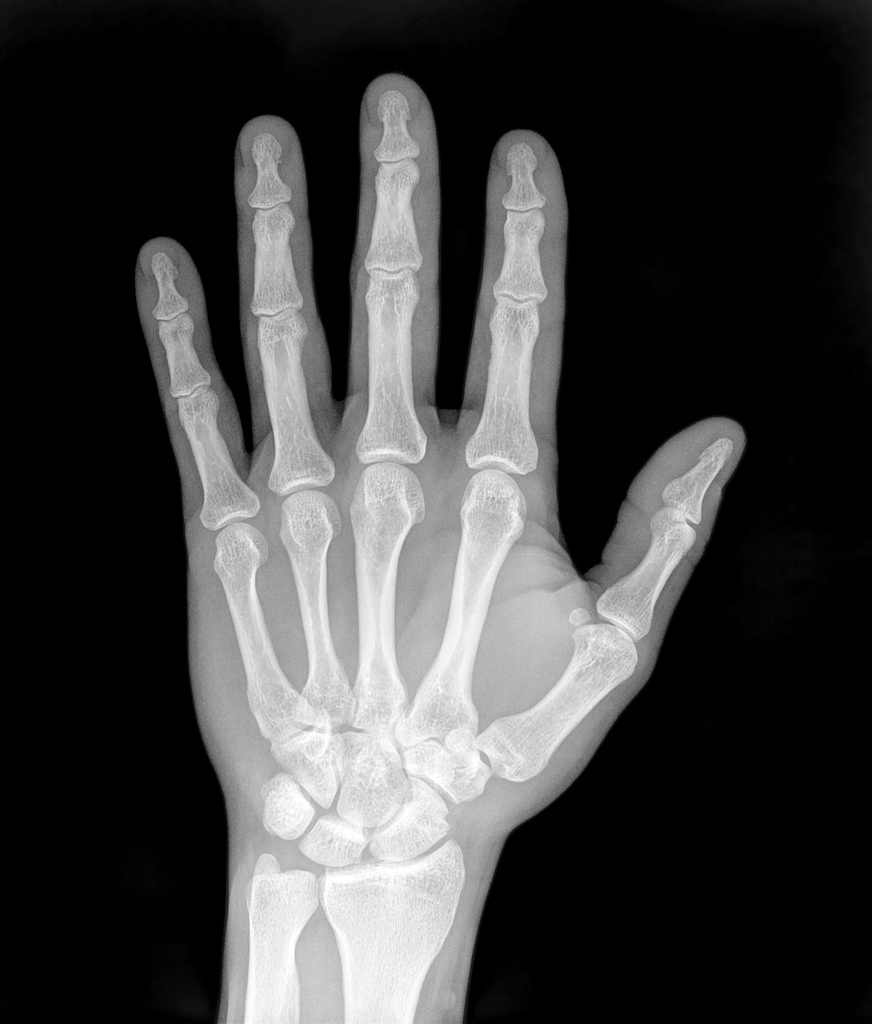
\includegraphics[width=0.8\textwidth]{photos/x-ray-hand_TraceMeek_flickr.jpg}\end{center}
\end{minipage}

            \subsubsection*{Selfone en Mikrogolf Bestraling}
            \nopagebreak
\begin{minipage}{.5\textwidth}
\includegraphics[width=.8\columnwidth]{photos/cellphones_kapungo.jpg}
\end{minipage}
\begin{minipage}{.5\textwidth}
            \label{m38779*id189654} Selfoon bestraling en gesondheids kwessies is al geopper, veral weens die enorme verhoging in selfoongebruik. Die rede agter die kommer is omdat selfone gebruik maak van elektromagnetiese golwe in die mikorgolf reeks. Hierdie kwessies het al gelei tot  'n groot volume van navorsing. Kommer oor die effek op gesondheid is ook al geopper rakende ander draadlose digitale stelsels, soos data kommunikasie netwerke. 
In 2009 het die Wereld Gesondheidsorganisasie aangekondig dat hulle  'n verband gevind het tussen brein kanker en selfone. Daar is egter nog nie konkrete bewyse vir hierdie stelling nie, en die verband is meestal vaag. Jy kan meer uitvind by: http://www.who.int/mediacentre/factsheets/fs193/en/\footnote{http://www.who.int/mediacentre/factsheets/fs193/en/}
        \par 
\end{minipage}
        \label{m38779*id189664} Selfoongebruikers word aangeraai om hul blootstelling aan bestraling te minimaliseer, deur byvoorbeeld:\par 
        \label{m38779*id189668}\begin{enumerate}[noitemsep, label=\textbf{\arabic*}. ] 
            \label{m38779*uid24}\item Die gebruik van  'n handvrye toestel ("hands-free") om die bestraling na die brein te laat afneem.
\label{m38779*uid25}\item Hou die selfoon weg van jou liggaam.
\label{m38779*uid26}\item Moenie  'n selfoon in  'n motor gebruik sonder  'n eksterne antenna nie. 
\end{enumerate}
        \label{m38779*uid27}
            \begin{exercises}{Penetrasie vermo\"ens van EM bestraling}
            \nopagebreak
        \label{m38779*id189729}\begin{enumerate}[noitemsep, label=\textbf{\arabic*}. ] 
            \label{m38779*uid28}\item Dui aan die penetrasie vermo\"ens van die verskillende tipes EM bestraling en koppel dit met die energie wat betrekking hou met die radiasie. \newline
\label{m38779*uid29}\item Beskryf die gevare van gamma-strale, x-strale and die skadelike effek van ulta-violet bestraling op jou vel. \newline
\end{enumerate}
    \label{m38779*cid8}
\practiceinfo
 \par \begin{tabular}[h]{cccccc}
 (1.) l2l  &  (2.) l2q  & \end{tabular}
\end{exercises}


            \section{Die partikel aard van elektromagnetiese bestraling}
            \nopagebreak
      \label{m38778*id188832} Wanneer ons praat van elektromagnetiese bestraling as  'n partikel, dan verwys ons na fotons, wat pakkies energie is. Die energie van die foton hou verband met die golflengte van die elektromagnetiese bestraling volgens:\par 
\label{m38778*fhsst!!!underscore!!!id476}\Definition{   \label{id2454271}\textbf{ Planck se konstante }} { \label{m38778*meaningfhsst!!!underscore!!!id476}
      \label{m38778*id188843}Planck se konstante is  'n fisiese konstante vernoem na Max Planck.\par 
      \label{m38778*id188849}$h=6,626\ensuremath{\times}{10}^{-34}$ J $\ensuremath{\cdot}$ s
 \par 
       } 
      \label{m38778*id188898} Die energie van  'n foton kan bereken word met die gebruik van die volgende formule: $E=hf$ or $E=h\frac{c}{\lambda }$.
Waar E die energie van die foton in joules is (J), h is planck se konstante, c is die spoed van lig, f is die frekwensie in hertz (Hz) en $\lambda $ is die golflengte in meters (m).\par Hoe hoer die frekwensie van die EM bestraling is, hoe hoer is die nergie gekoppel daaraan.  
      \begin{wex}
      {Die berekening van die energie van  'n foton I
      }
      {
      \label{m38778*id188962} Bereken die energie van  'n foton met  'n frekwensie van $3\ensuremath{\times}{10}^{18}$~Hz}
      {
  \westep{Pas die formule toe vir die energie van  'n foton.}
    \begin{eqnarray}
    E& =& hf\\ 
     & =& 6,6\ensuremath{\times}{10}^{-34}\ensuremath{\times}3\ensuremath{\times}{10}^{18}\\ 
     & =& 2\ensuremath{\times}{10}^{-15}\phantom{\rule{0.166667em}{0ex}}\text{J}
     \end{eqnarray}
      }
      \end{wex}
    
  \begin{wex}{Die berekening van die energie van  'n foton II}{Wat is die energie van  'n ultra-violet foton met  'n golflengte van 200~nm?}{
      \label{m38778*id189184}Ons word vereis om die energie geassosieerd met  'n ultra-violet foton met  'n golflengte van 200~nm te bereken.\par 
      \label{m38778*id189190}Ons kan dievolgende gebruik:\par 
      \label{m38778*id189193}\nopagebreak\noindent{}
        
    \begin{equation}
    E=h\frac{c}{\lambda }
      \end{equation}
      \label{m38778*id189220}\nopagebreak\noindent{}
    
    \begin{equation}
    \begin{array}{ccc}\hfill E& =& h\frac{c}{\lambda }\hfill \\ & =& \left(6,626\ensuremath{\times}{10}^{-34}\right)\frac{3\ensuremath{\times}{10}^{8}}{200\ensuremath{\times}{10}^{-9}}\hfill \\ & =& 9,939\ensuremath{\times}{10}^{-10}\phantom{\rule{0.166667em}{0ex}}\text{J}\hfill \end{array}
      \end{equation}}
         \end{wex}
      \label{m38778*uid13}
            \begin{exercises}{Partikel aard van EM golwe}
            \nopagebreak
        \label{m38778*id189384}\begin{enumerate}[noitemsep, label=\textbf{\arabic*}. ]
            \label{m38778*uid14}\item Wat is die verband tussen die energie van  'n foton met die frekwensie en die golflengte van die foton? \newline
\label{m38778*uid15}\item Bepaal die energie van  'n foton (EM bestraling) met  'n frekwensie van ${10}^{12}$~Hz.\newline
\label{m38778*uid16}\item Bepaal die energie van  'n foton (EM bestraling) met  'n golflengte van 600 nm.\newline
\end{enumerate}
  \label{m38778**end}
\practiceinfo
 \par \begin{tabular}[h]{cccccc}
 (1.) l2H  &  (2.) l26  &  (3.) l2F  & \end{tabular}
\end{exercises}
            
    \label{m38779*eip-745}
            \subsection*{Gedrag van Diere}
            \nopagebreak
            \label{m38779*id1164126080746} Mense glo al vir eeue dat diere kan aanvoel wanneer  'n aardbewing of ander natuurramp op hande is. Reeds in 373 V.C, het historici al opgeteken rakende massiewe uittogte van diere, insluitende rotte, slange en meerkatte wat gevlug het uit die Griekse stad Helice etlike dae voor  'n aardbewing getref het, wat groot skade aangerig het.  \par 
      \label{m38779*id1164126439136} Hierdie onderwerp is al baie gedebatteer, en verskillende gedragspatrone word gevind by verskillende diere, byvoorbeeld: \par 
      \label{m38779*id1164132827593}\begin{itemize}[noitemsep]
            \item \textbf{Honde en katte}: honde en katte tjank rondom en byt selfs glo hul eienaars net voor  'n natuurramp, en die eienaars voer aan dat die diere se verhoogde reuksintuig daartoe lei.
\item \textbf{Haaie}: navorsers in Florida het al aangedui dat haaie beweeg na dieper water voordat orkane tref, waarskynlik weens  'n sensitiwiteit vir die verandering in die lugdruk net voor die orkaan tref. 
\item \textbf{Knaagdiere}: knaagdiere wat ondergrond woon, sal baie keer uit hul gate vlug voor  'n ramp tref. Wetenskaplikes van Caltech het al gevind dat daar baie veranderings is wat  'n aardbewing voorafgaan, byvoorbeeld  'n verandering in die aarde se oppervlak. Knaagdiere is meermale meer sensitief teenoor sulke klein veranderings en sal gevolglik daarop reageer. 
\item \textbf{Olifante}: sal blykbaar trompetter en vlug na hoogliggende gebiede voor  'n tsunami sy opwagting maak. Hierdie gedrag word toegeskryf aan hul sensitiwiteit vir vibrasies op die Aarde se oppervlak. \end{itemize}
      \label{m38779*id1164121170251}Baie navorsings debatteer dat diere sekere natuurlike seine kan aanvoel, soos die vooraf trillings van  'n aardbewing. Dit beteken dat die diere het die geleentheid om te reageer voordat mense kan. Dit moet egter bygese word dat die diere nie noodwendig verstaan waarom hulle so instinktief optree nie. Hulle vlug net soos enige mens sou vlug as iemand "Brand!" sou skreeu. \par 
      \label{m38779*id6489198}  'n Verdere probleem wat gemeld word net hierdie klaarblyklike heldersiende diere is dat hul psigiese gedrag dikwels gebasseer is op gedrag wat mense eers herroep na die gebeurtenis. Sommige dierlike gedrag gebeur gereeld, maar word nie onthou tensy  'n aardbewing, tsunami of modderstorting volg nie. Byvoorbeeld, as jy  'n hond  'n pad sien oorsteek, sal jy slegs onthou dat jy  'n hond  'n pad sien oorsteek het. Maar as  'n aardbewing jou area 5 minute later getref het, sou jy dink die hond het gevlug?  \par 
      \label{m38779*id1553831}
            \begin{project}{Diere en natuurlike rampe}
            \nopagebreak
        \label{m38779*id1164119615164} Doen navorsing oor die gedrag van diere net voor  'n natuurramp tref. \par 
        \label{m38779*id1164121934705} Kies een tipe natuurramp (aardbewing, vloed, tsunami, ens.) en kyk wat jy kan opspoor oor hoe diere reageer teenoor hierdie betrokke tipe ramp. Vra vir mense wie jy ken wat hulle al gehoor het rakende hierdie tipe verhale.\par 
        \label{m38779*id1164121037612} Vors daarna die onderwerp na, ten einde meer informasie te bekom, en onthou om alle informasie krities te benader. Dinge om te oorweeg: \par 
        \label{m38779*id1164128014077}\begin{itemize}[noitemsep]
            \item Watter wetenskaplike navorsing is al gedoen?   
\item In watter lande vind die natuurramp gewoonlik plaas? 
\item Is daar enige van die natuurlike inwoners van daardie land wat stories het oor hoe die diere reageer op so  'n natuurramp?  
\item Wat glo mense lei tot hierdie gedrag? Bv. het die diere  'n magiese krag of is hulle meer sensitief rakende hierdie gebeure as ons, met betrekking tot lae frekwensie bestraling? \end{itemize}
Sommige voorgestelde bronne vir informasie sluit in:
\begin{itemize}[noitemsep]
\item \textsl{http://www.unep.org/ik/}
\item \textsl{http://earthquake.usgs.gov/learn/topics/animal\_eqs.php}
\item \textsl{http://biology.about.com/od/animalbehavior/a/aa123104a.htm} 
\item \textsl{http://news.nationalgeographic.com/news/2003/11/1111\_031111\_earthquakeanimals\_2.html}
\item \textsl{Bats sing, mice giggle} deur Karen Shanor en Jagmeet Kanwal
\item \textsl{http://www.sheldrake.org/homepage.html}
\item \textsl{http://nationalzoo.si.edu/SCBI/AnimalCare/News/earthquake.cfm}
\item \textsl{http://www.animalvoice.com/animalssixthsense.htm}
\end{itemize}
        \label{m38779*id1164121076422} Vertel jou klas van jou bevindings. Analiseer jou versamelde informasie krities en besluit wat jy gaan glo\par 
      \label{m38779*cid9}
      \end{project}

\summary{VPfhw}

            \nopagebreak
      \label{m38779*id189769}\begin{enumerate}[noitemsep, label=\textbf{\arabic*}. ] 
            \label{m38779*uid30}\item Elektromagnetiese bestraling het beide  'n golf en partikel geaardheid.
\label{m38779*uid31}\item Elektromagnetiese golwe beweeg teen  'n spoed van $3\ensuremath{\times}{10}^{8}\phantom{\rule{3.33333pt}{0ex}}m\ensuremath{\cdot}{s}^{-1}$ in  'n vakuum.
\label{m38779*uid32}\item Die Elektromagnetiese spektrum bestaan uit die volgende tipes bestraling: radio golwe, mikro-golwe, infra-rooi golwe, sigbare golwe, ultra-violet golwe, x-strale en gamma-strale. 
\label{m38779*uid33}\item Gamma-strale het die meeste energie en het die hoogste penetrasie vermoens, terwyl radio-golwe die minste energie besit en die mins penetrerende is. 
\end{enumerate}
            \begin{eocexercises}{Einde van die hoofstuk oefening}
            \nopagebreak
      \label{m38779*id189872}\begin{enumerate}[noitemsep, label=\textbf{\arabic*}. ] 
            \label{m38779*uid34}\item Bepaal die energie van  'n foton (EM bestraling) met  'n frekwensie van $3\ensuremath{\times}{10}^{8}$~Hz?\newline
\label{m38779*uid35}\item Bepaal die energie van  'n lig foton met  'n golflengte van 660~nm?\newline
\label{m38779*uid36}\item Lys die hoof tipes elektromagnetiese bestraling in volgorde van toenemende golflengte.\newline
\label{m38779*uid37}\item Lys die hoof gebruike van:
\label{m38779*id189946}\begin{enumerate}[noitemsep, label=\textbf{\alph*}. ] 
            \label{m38779*uid38}\item radio golwe
\label{m38779*uid39}\item infra-rooi strale
\label{m38779*uid40}\item gamma-strale
\label{m38779*uid41}\item X-strale
\end{enumerate}
                \label{m38779*uid42}\item Verduidelik waarom ons onsself moet beskerm teen ultra-violet bestraling van die son. \newline
\label{m38779*uid43}\item Lys  'n paar voordele en nadele van x-strale se gebruik. \newline
\label{m38779*uid44}\item Watter voorsorg behoort mens te tref indien jy  'n selfoon gebruik? \newline
\label{m38779*uid45}\item Skryf  'n kort opsomming oor die tipes elektromagnetiese golwe. Jy moet insluit die gebruike, voordele en nadele van jou gekose bestraling opsies.\newline
\label{m38779*uid46}\item Veruidelik waarom sekere tipes bestraling hoer penetrasie vermo\"ens as ander het.\newline
\end{enumerate}
  \label{m38779**end}
  \label{459e2bef85baf867f5850bc8338cad3a**end}
\practiceinfo
 \par \begin{tabular}[h]{cccccc}
 (1.) l4J  &  (2.) l4u  &  (3.) l2r  &  (4.) l21  &  (5.) l2Y  &  (6.) l4h  &  (7.) l4S  &  (8.) l24  &  (9.) l2g  & \end{tabular}
\end{eocexercises}
